\subsection{Gain allocation functions}

At this stage, we have a model that let us operates the community in a fully centralized way as well as in a fully decentralized way. This way we can compute the gain of the community by comparing the cost of the community in the centralized case with the cost of the community in the decentralized case. As the model in the centralized case hold more information and does not add constraints that will affect the objective cost negatively, we can be sure that the cost of the community in the centralized case will be lower than the cost of the community in the decentralized case. Thus, we can be sure that the gain of the community will be positive. We can then define a gain allocation vector $x$ that will give to each member of the community a share of the gain. So we should have :
\begin{align}
    &Gain = Objective_{centralized} - \sum_{i \in M} Objective_{centralized,i} \\
    &\sum_{i \in M} x_i = Gain
\end{align}
With M the set of members of the community, $Objective_{centralized}$ the value of the objective function in the centralized case, and $Objective_{centralized,i}$ the value of the objective function for member i in the centralized case.

For this, we will use the functions defined in the state of the art section \ref{section_allocation}. As said in \ref{methodology}, we will use the Shapley value defined in equation \ref{eq:shapley}, the proportional allocation defined in equation \ref{eq:PA}, and an egalitarian allocation defined as follows:
\begin{equation}
    x_i = \frac{Gain}{|M|}
\end{equation}
With $|M|$ the number of members in the community. 

Of course, it does not make sense to allocate environmental gains or comfort gains without changing the operation of the community. So when allocating the gains, we will only talk about the economic gains. But we can still compute the proportional allocation and Shapley value using the total objective gain in order to consider the contribution of each member for the total objective of the community.

The full optimization process is shown in figure \ref{fig:gain_allocation}. 

\begin{figure}[ht]
    \centering
    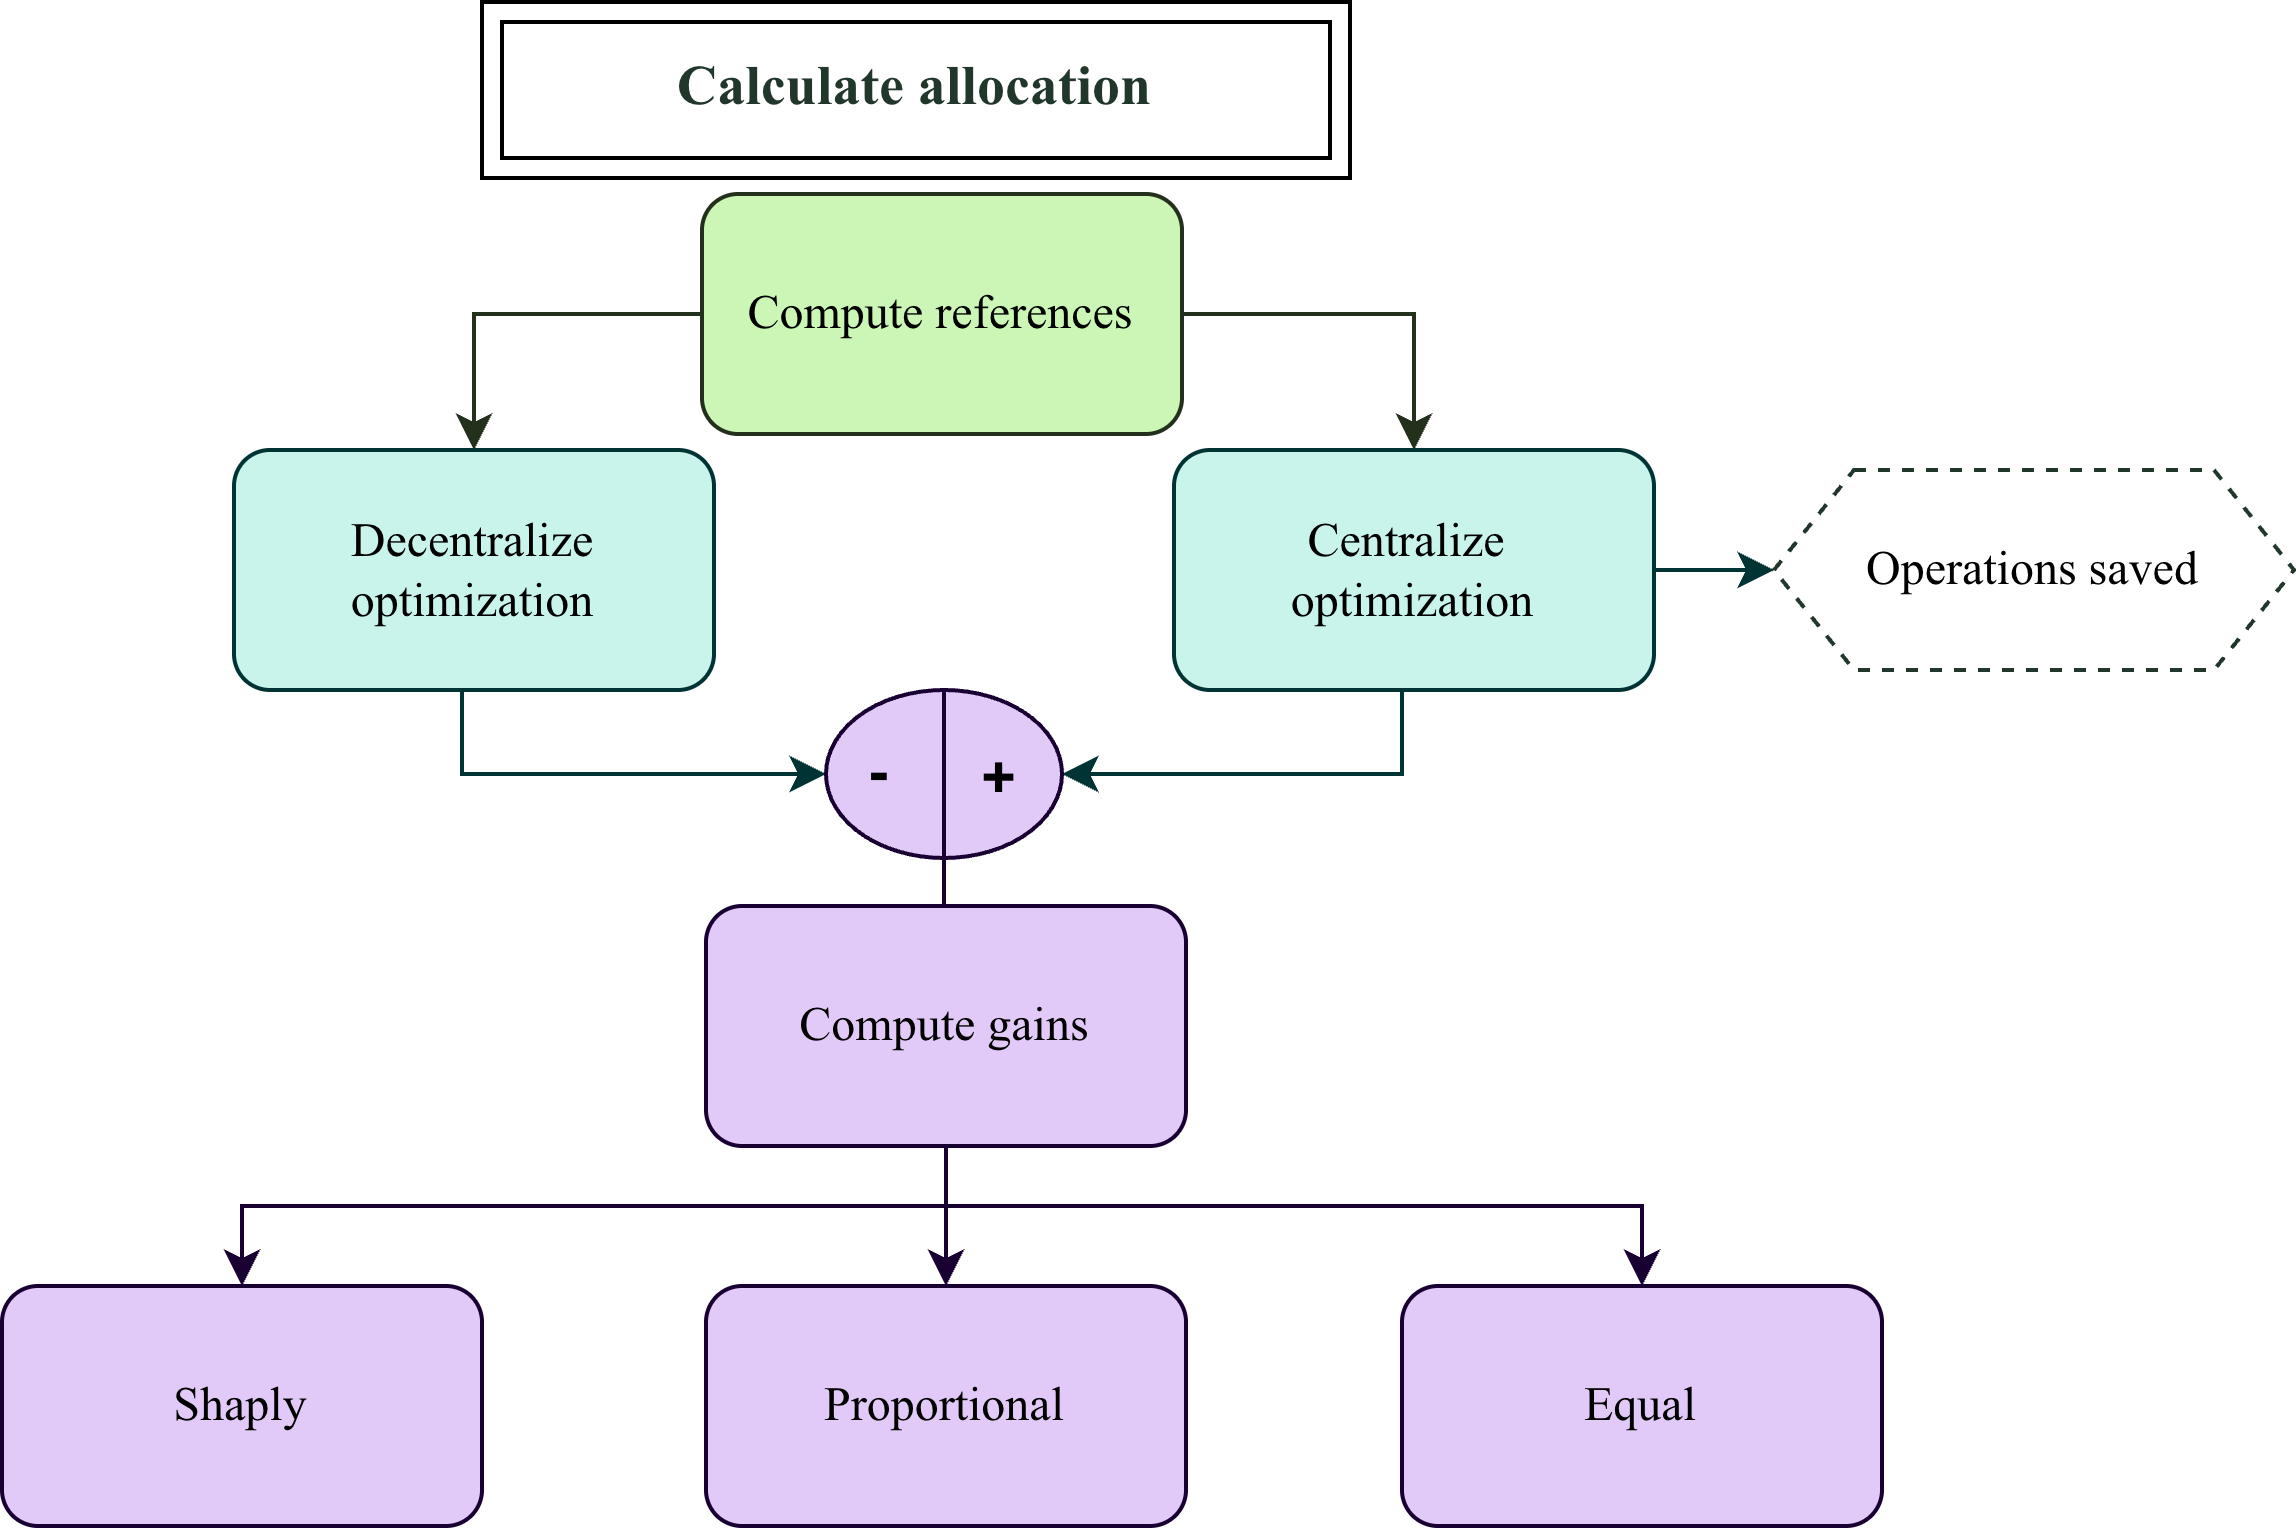
\includegraphics[width=0.6\textwidth]{allocation_schema.png}
    \caption{Gain allocation process}
    \label{fig:gain_allocation}
\end{figure}
